	% Set document type and scheme
	\documentclass[10pt]{beamer}
	\usetheme[progressbar=frametitle]{metropolis}


	% Load packages
	\usepackage{lmodern}
	\usepackage{appendixnumberbeamer}
	\usepackage{booktabs}
	\usepackage[scale=2]{ccicons}
	\usepackage{pgfplots}
	\usepackage{xspace}
		\newcommand{\themename}{\textbf{\textsc{metropolis}}\xspace}
	\usepackage{stata}
	\usepackage{graphicx}

	\title{Stata Workshop} %% that will be typeset on the
	\subtitle{At MINAGRI} %% title page.
	\author{Roshni Khincha and Sakina Shibuya \\ DIME, World Bank}
	\date{August, 2018}

	\titlegraphic{%
		
\includegraphics[width=.2\textwidth]{DIME}\hfill % I think I should probably ask for a better image for this thing....
		
\includegraphics[width=.15\textwidth]{logo_minagri}\hfill
		
\includegraphics[width=.2\textwidth]{logo_eu}
		}

	\makeatletter
	\setbeamertemplate{title page}{
		\begin{minipage}[b][\paperheight]{\textwidth}
			\vfill%
			\ifx\inserttitle\@empty\else\usebeamertemplate*{title}\fi
			\ifx\insertsubtitle\@empty\else\usebeamertemplate*{subtitle}\fi
			\usebeamertemplate*{title separator}
			\ifx\beamer@shortauthor\@empty\else\usebeamertemplate*{author}\fi
			\ifx\insertdate\@empty\else\usebeamertemplate*{date}\fi
			\vfill
			\ifx\inserttitlegraphic\@empty\else\inserttitlegraphic\fi
			\vspace*{1cm}
		\end{minipage}
		}
	\makeatother

	\begin{document}
		
	\maketitle

	\section{Section 1}
	\section{Section 2}

	\begin{frame}
	\frametitle{\textsc{Edit data in Stata}}
\begin{stlog}tabulate s5bq3a
summarize s5bq3a 
codebook s5bq3a
\end{stlog}
	\end{frame}
	
	\begin{frame}
	\frametitle{\textsc{Lab Task 7: Saving Stata datasets}}	
		\begin{itemize}
			\item The command for saving a Stata dataset is \textit{\textbf{save}}.
			\item \textit{save} saves your data in memory in a file format called dta. 
				  This is a file that can only be read with Stata.
			\item The command for saving a dataset in excel and csv is \textit{\textbf{export}}.
			\item \textit{\textbf{export}} is the opposite of import, and is very versatile. 
				  It lets you save data in excel, csv, sas and others. 
				  Please refer to the help file on \textit{\textbf{export}}.
		\end{itemize}	
	\end{frame}

	\begin{frame}
	\frametitle{\textsc{Lab Task 7: Saving Stata datasets}}	
		\begin{columns}
			\begin{column}{0.5\textwidth}
				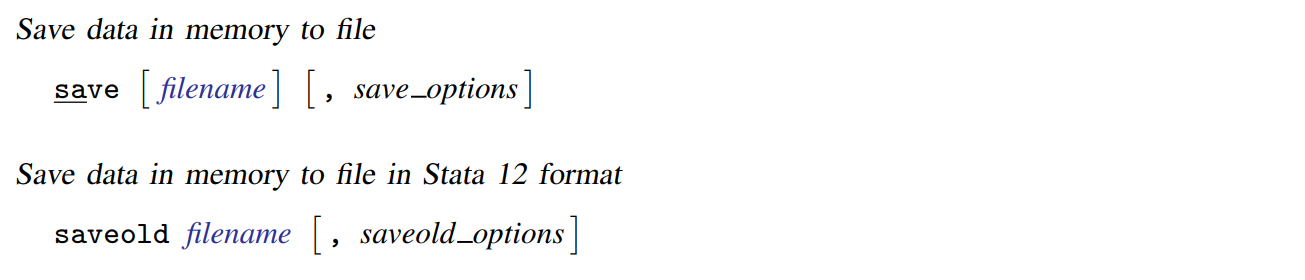
\includegraphics[width=\linewidth]{helpfile_save_1}
				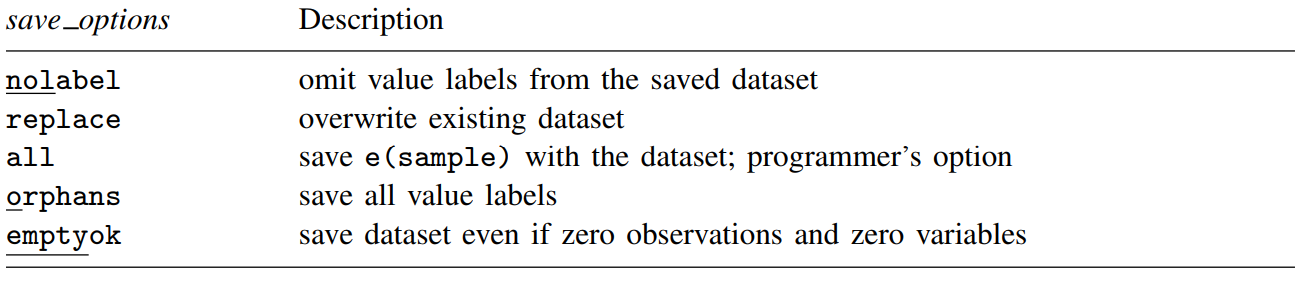
\includegraphics[width=\linewidth]{helpfile_save_2}
			\end{column}
			\begin{column}{0.5\textwidth}
				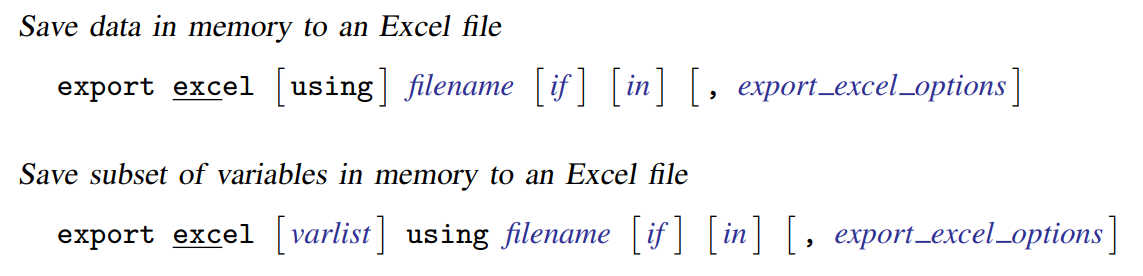
\includegraphics[width=\linewidth]{helpfile_exportexcel_1}
				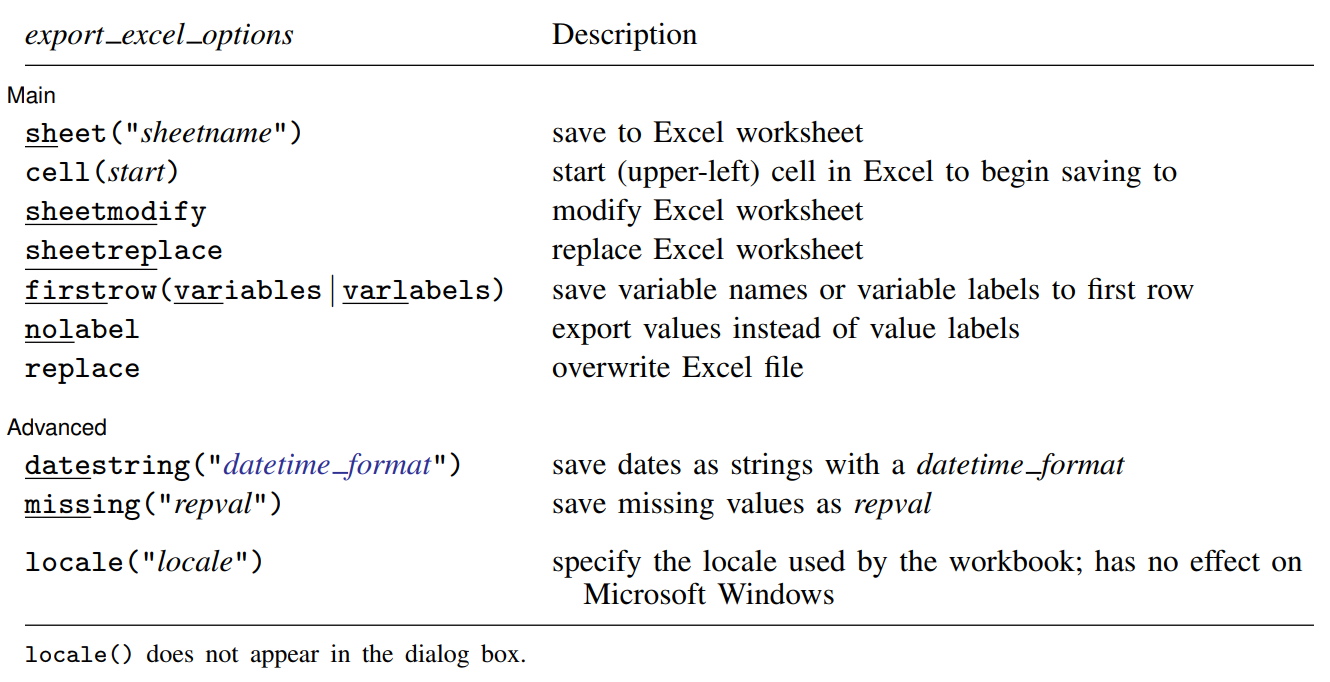
\includegraphics[width=\linewidth]{helpfile_exportexcel_2}
			\end{column}
		\end{columns}
	\end{frame}
	
	\begin{frame}
		\frametitle{\textsc{Lab Task 7: Saving Stata datasets}}	
		\onslide<1-> Let's save the modified data as a dta file.
					\vspace{2mm} Type...
\begin{stlog}. tabulate ur2012 
\end{stlog}
		\vspace{2mm}
		\onslide<2-> Notice that we use the \textbf{\textit{replace}} option. 
					 This overwrites the existing file. 
					 \vspace{2mm} Type the same command without \textbf{\textit{, replace}}, 
					 and see what error you get! 
		\vspace{2mm}			 
		\onslide<3-> Did you get an error like this? 
		\begin{center}			
			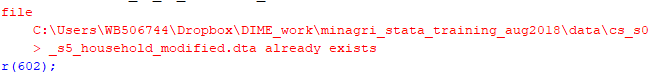
\includegraphics[width=0.8\linewidth]{error_save_existing}
		\end{center}
	\end{frame}
	
	\begin{frame}
		\frametitle{\textsc{Lab Task 7: Saving Stata datasets}}
		\onslide<1-> Now, let's save the modified data as a excel. 
					 This is helpful if you are sending the dataset to 
					 someone who does not use or have Stata. \\
					 Type...
		\vspace{2mm}
\begin{stlog}. use "$data\\cs_s0_s5_household.dta", clear
{\smallskip}
\end{stlog}
		\vspace{2mm}
		\onslide<2-> Open the output file. 
					 Notice that it doesn't have variable names as column names.
					 This is very inconvenient!
		\onslide<3-> Use an optional command, \textbf{\textit{firstrow(variables)}}.
		\vspace{2mm}
\begin{stlog}. keep hhid province district ur2012 s5cq2 s5cq4 s5cq8 s5cq15 s5cq23 s5bq2 s5cq22 s5cq1
> 3 s5cq17 
{\smallskip}
\end{stlog}
		\vspace{2mm}
		\onslide <4-> Notice \textbf{///}. This is a way to let Stata now that multiple lines
					  constitute a single command. It's helpful when your command is getting too
					  long on your do file.
		\onslide<5-> Open the newly saved excel file. You will find column names!
	\end{frame}
	
	
	\section{Section 3: \\ Introduction to Stata Graphics}
	
	\begin{frame}
	\frametitle{\textsc{Table gives all the details.}}
		\begin{center}
		What's happening in this regression table? What's important?
		\begin{figure}
			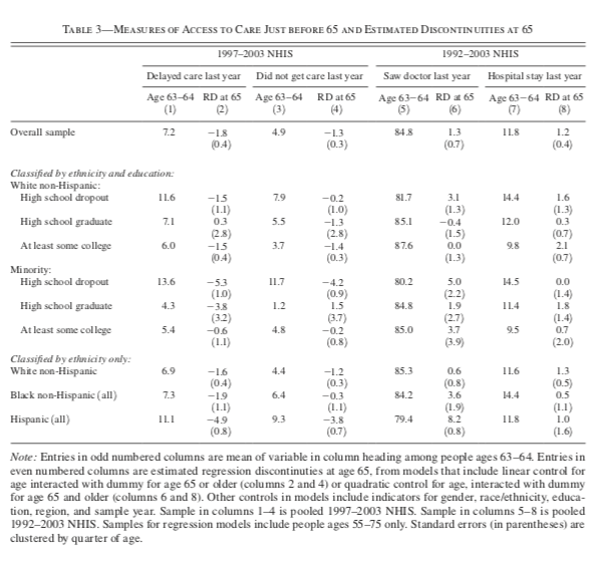
\includegraphics[width=0.7\linewidth]{reg_table_example}
		\end{figure}		
		\end{center}
	\end{frame}

	\begin{frame}
	\frametitle{\textsc{But figures \textit{tell the story}.}}
		\begin{columns}
			\column{0.55\linewidth}
			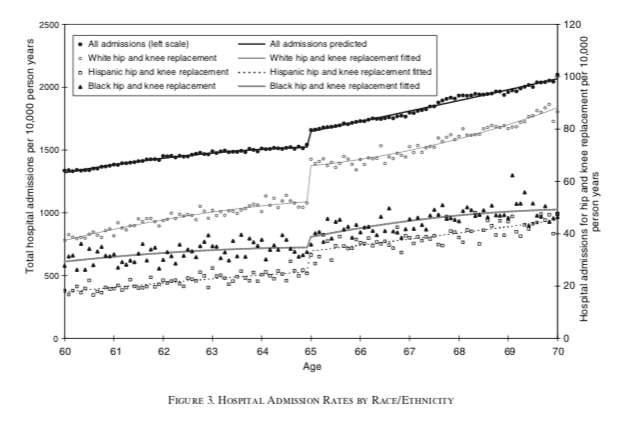
\includegraphics[height=5cm, width=6cm]{figure_example_1}
			\hspace{5mm}
			\column{0.45\linewidth}
			\begin{itemize}
				\item This is the data that generates those estimates.
				\item You can see exactly what is happening very quickly!
				\item Even more importantly: \\ \textbf{Your eyes are naturally drawn to the story!}
			\end{itemize}
		\end{columns} 
	\end{frame}

	\begin{frame}
	\frametitle{\textsc{Example: comparing means}}
		\begin{columns}
		\column{0.55\linewidth}
		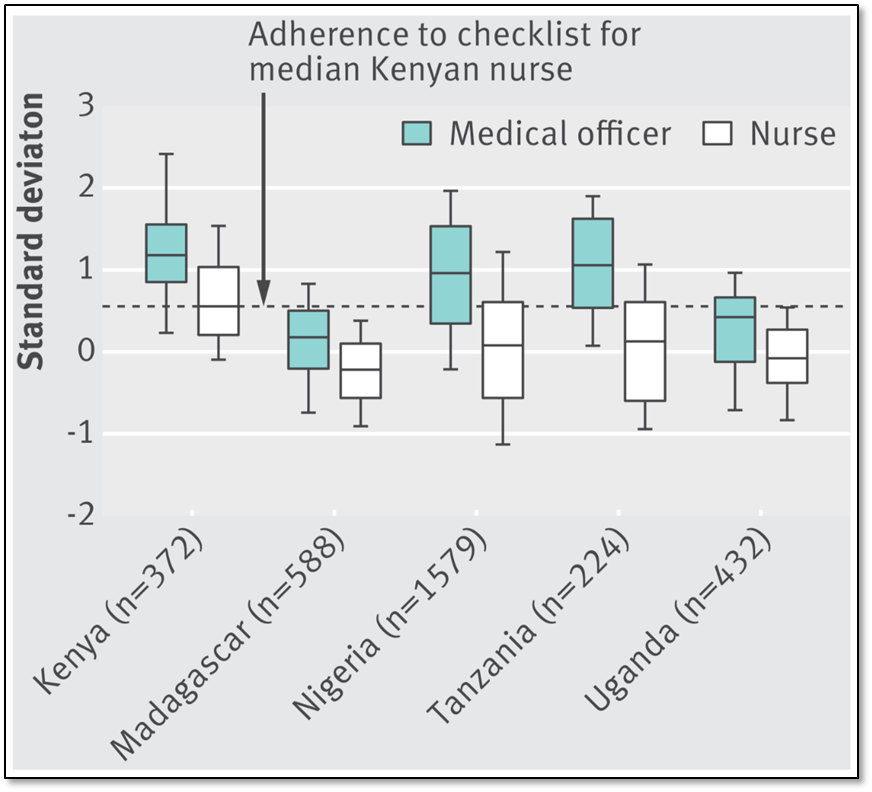
\includegraphics[height=5cm, width=6cm]{figure_example_2}
		\hspace{5mm}
		\column{0.45\linewidth}
		\begin{itemize}
			\item What is the main story in this graph? 
			\item We need more context to say something detailed about this, 
				  but what has the person creating the graph highlighted for us?
		\end{itemize}
		\end{columns} 
	\end{frame}
	
	
	\begin{frame}
	\frametitle{\textsc{Stata default graphs}}
		\begin{itemize}
			\item This is what a Stata graph looks like with very minimal 
				  customizing using optional commands.
			\item Notice that there is no graph title. 
				  They are still informative, but need much improvement.
			\item We will not go too deep to editing a Stata graph today,
				  but I'll show you have to make a graph and make some edits
				  for effective data visualization.
		\end{itemize}	
		\begin{center}
			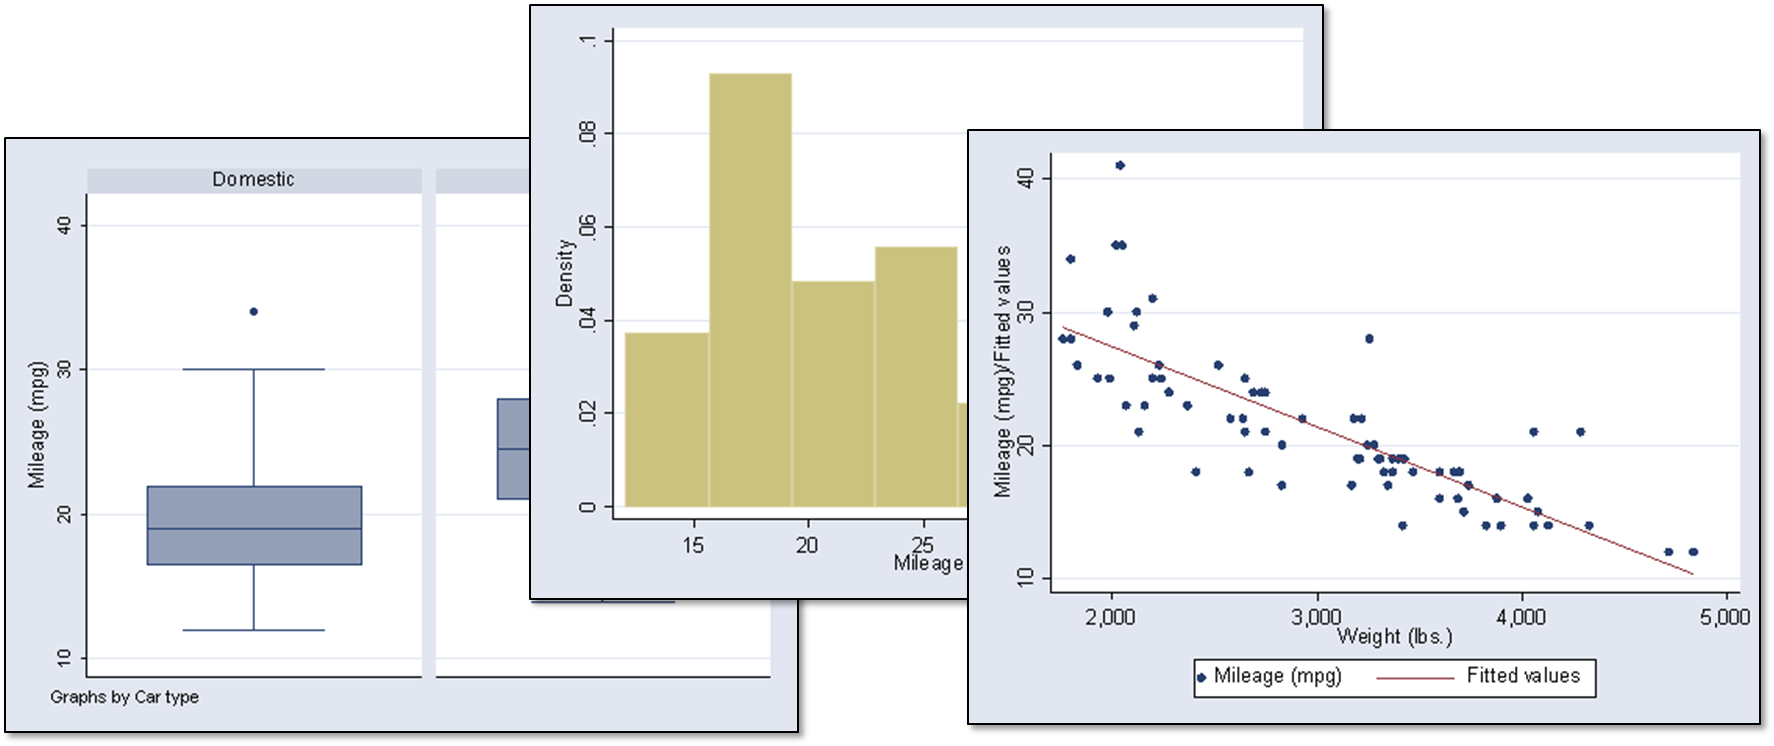
\includegraphics[width=\linewidth]{figure_example_3}
		\end{center}
	\end{frame}

	\begin{frame}
	\frametitle{\textsc{Stata has three core built-in graph functions.}}
		\begin{columns}
			\column{0.4\linewidth}
			\textbf{[graph \textit{graphtype}]} \\
			\small graphs which plot one or more variables on one axis \\ \vspace{2mm}
			\textbf{[twoway \textit{graphtype}]} \\
			\small graphs which plot two variables together on an x and y axis \\  \vspace{2mm}
			\small \textbf{\textit{twoway\_options}} is a set of optional commands that can be
					applied to all twoway graphs. \\
			\textbf{[histogram], [kdensity], [lowess]} \\
			\small Essential distributional commands
			\column{0.6\linewidth}
			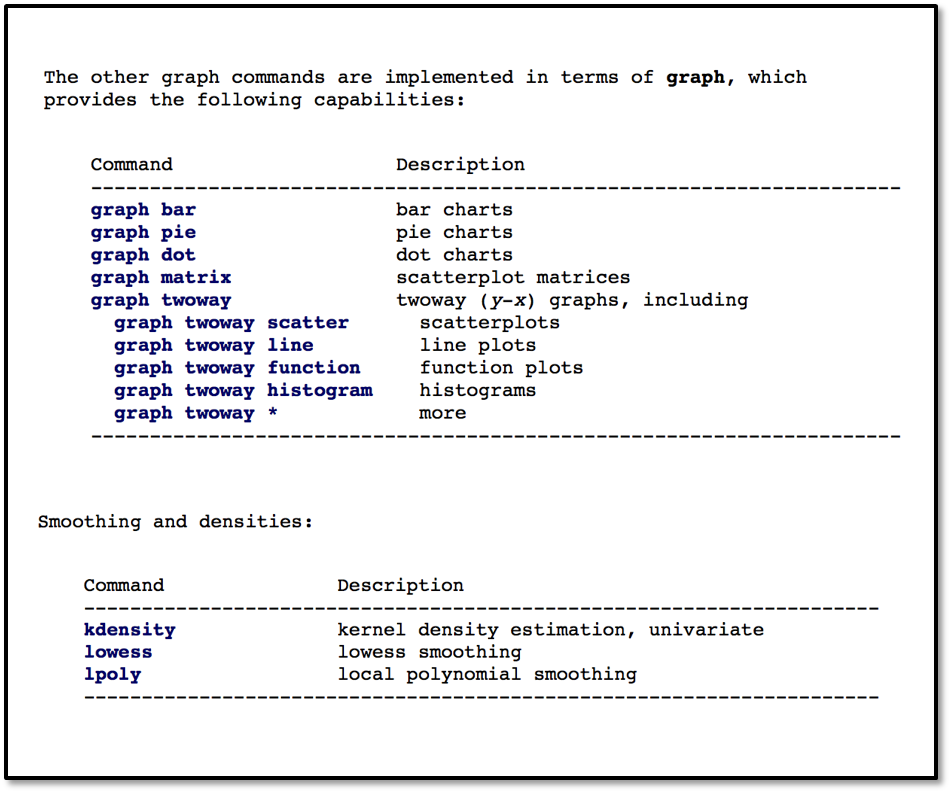
\includegraphics[height=6cm, width=7cm]{stata_builtin_graph_functions}
		\end{columns}
	\end{frame}
	
	\begin{frame}
	\frametitle{\textsc{Stata graph exercise 1}}
		\begin{center}
		\Large \textbf{Box plot}
		\end{center}
	\end{frame}	

	\begin{frame}
	\frametitle{\textsc{Box plot}}
		Let's make a a box plot like the one below using the variable, \textbf{m\_drink\_ws}.
		Notice a box plot is an example of a oneway graph. 
\begin{center}
    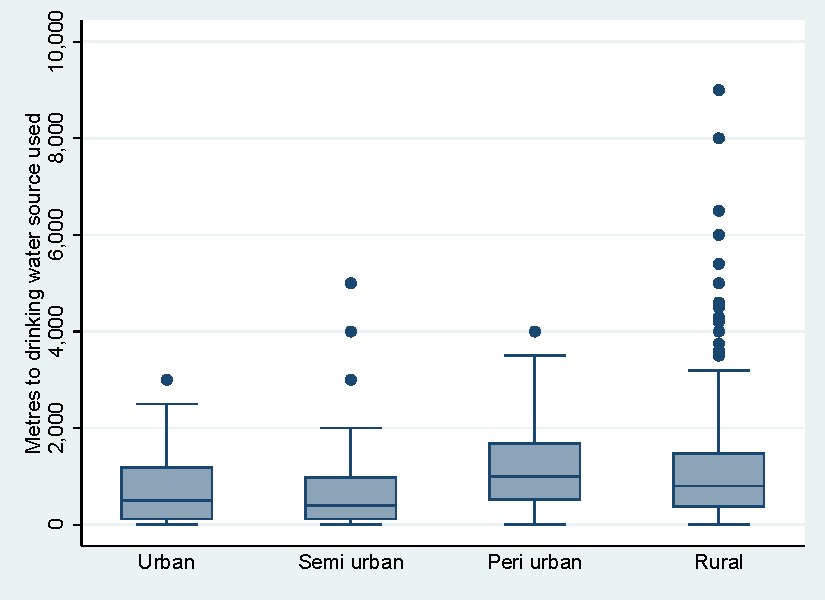
\includegraphics[width=0.8\textwidth]{boxplot_1.pdf}
\end{center}
	\end{frame}
	
	\begin{frame}
	\frametitle{\textsc{Box plot}}	
		\onslide<1-> Let's make a box plot from your do file.
		\begin{enumerate}
			 \item Type \textbf{\textit{search box plots}} in the command window to find out what command to be used.
					\textbf{\textit{search}} is a more general search through help files and other Stata resources.
			 \onslide<2-> \item The command should look like the following. Run from the do file.
		
\begin{stlog}generate  cm_main_ws = m_main_ws*100
\end{stlog}
			\vspace{2mm}
			\onslide<3-> \item Notice the difference from earlier? 
			\vspace{2mm}			
		
\begin{center}
    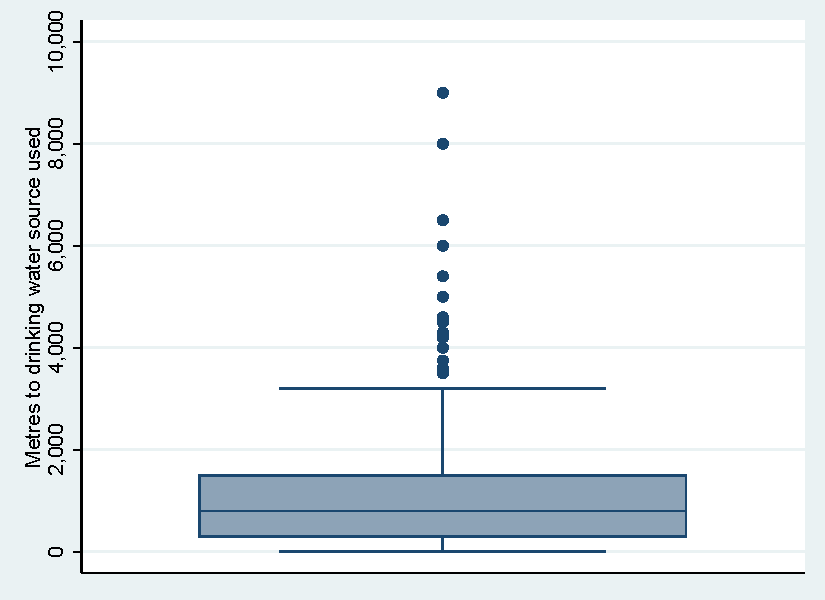
\includegraphics[width=0.5\textwidth]{boxplot_2.pdf}
\end{center}
		\end{enumerate}
	\end{frame}

	\begin{frame}
	\frametitle{\textsc{Box plot}}	
		\onslide<1-> Now, let's make multiple box plots by the residential environment, \textbf{urban\_2012}.
		\begin{enumerate}
			 \item Type \textbf{\textit{search box plots}} to see how to achieve this.
			 \onslide<2-> \item The optional commant, \textbf{\textit{over()}} can do this.
								Run the new \textbf{\textit{graph box}} command with the \textbf{\textit{over}} option.
		
\begin{stlog}. gen  d_closest_ws        = 0
{\smallskip}
\end{stlog}
\begin{center}
    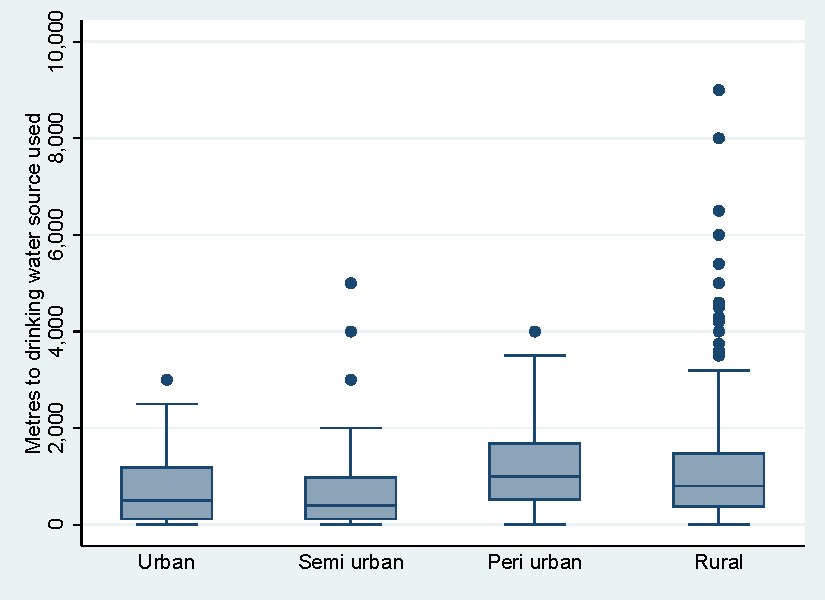
\includegraphics[width=0.5\textwidth]{boxplot_1.pdf}
\end{center}
		\end{enumerate}
	\end{frame}

	\begin{frame}
	\frametitle{\textsc{Stata graph exercise 2}}
		\begin{center}
		\Large \textbf{Histogram}
		\end{center}
	\end{frame}		
	
	\begin{frame}
	\frametitle{\textsc{Histogram}}
		Let's make a a histogram like the one below using the variable, \textbf{m\_drink\_ws}.
		Notice that a histogram is an example of a twoway graph.
	
\begin{center}
    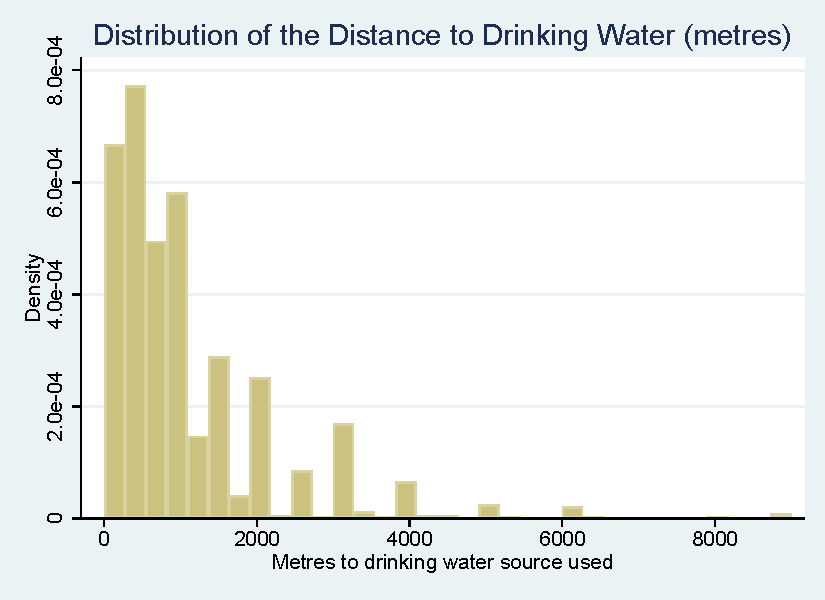
\includegraphics[width=0.8\textwidth]{hist_1.pdf}
\end{center}
	\end{frame}
	
	\begin{frame}
	\frametitle{\textsc{Histrogram}}	
		\onslide<1-> Let's make a histogram from your do file.
		\begin{enumerate}
			 \item Type \textbf{\textit{help histogram}} in the command window to find out what command to be used.
			 \onslide<2-> \item The command should look like the following. Run from the do file.
		
\begin{stlog}label define yes_no_lb 1 "Yes" 0 "No"
label values d_closest_ws yes_no_lb
\end{stlog}
			\vspace{2mm}
			\onslide<3-> \item Notice the difference from earlier? We need the title.
			\vspace{2mm}
		
\begin{center}
    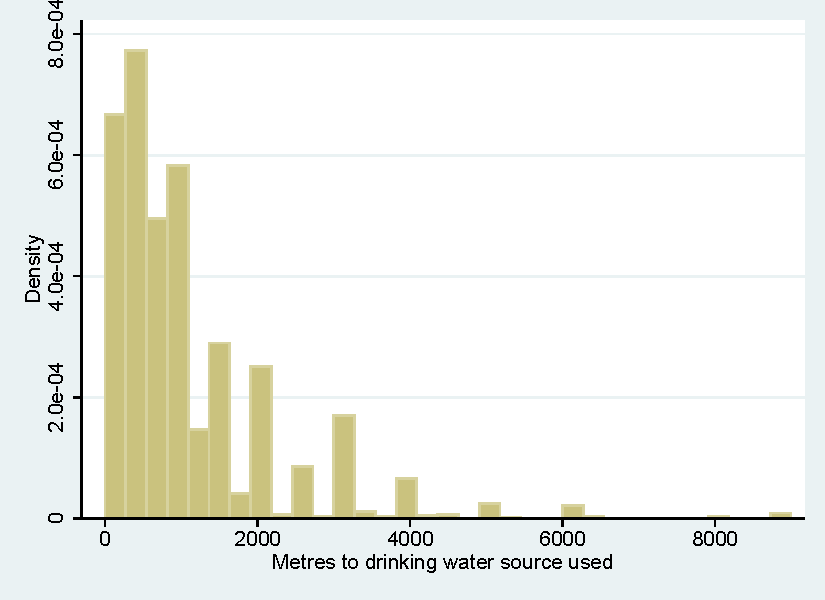
\includegraphics[width=0.5\textwidth]{hist_2.pdf}
\end{center}
		\end{enumerate}
	\end{frame}

	\begin{frame}
	\frametitle{\textsc{Histrogram}}	
		\onslide<1-> Now, let's add the title. You can also choose your own title that is informative.
					 Notice in general a good title is informative but short.
		\begin{enumerate}
			 \onslide<2-> \item The optional command, \textbf{\textit{title()}} can do this.
								Run the new \textbf{\textit{histogram}} command with 
								the \textbf{\textit{title}} option.
		
\begin{stlog}. global  data "$dropbox\\minagri_stata_training_aug2018\\data"
{\smallskip}
\end{stlog}
			\vspace{1mm}
			\onslide <4-> \item \textbf{\textit{help twoway\_options}} to find out more about the \textbf{\textit{title}} option and more.
		\end{enumerate}
	\end{frame}
	
	\begin{frame}
	\frametitle{\textsc{Stata graph exercise 3}}
		\begin{center}
		\Large \textbf{Scatter plot}
		\end{center}
	\end{frame}		
	
	\begin{frame}
	\frametitle{\textsc{Scatter plot}}
		Let's make a a scatter plot with a fitted line like the one below using the variable, \textbf{m\_drink\_ws} and \textbf{m\_used\_ws}.
		Notice that a scatter plot with a fitted line is an example of a twoway graph.
		\vspace{1mm}
	
\begin{center}
    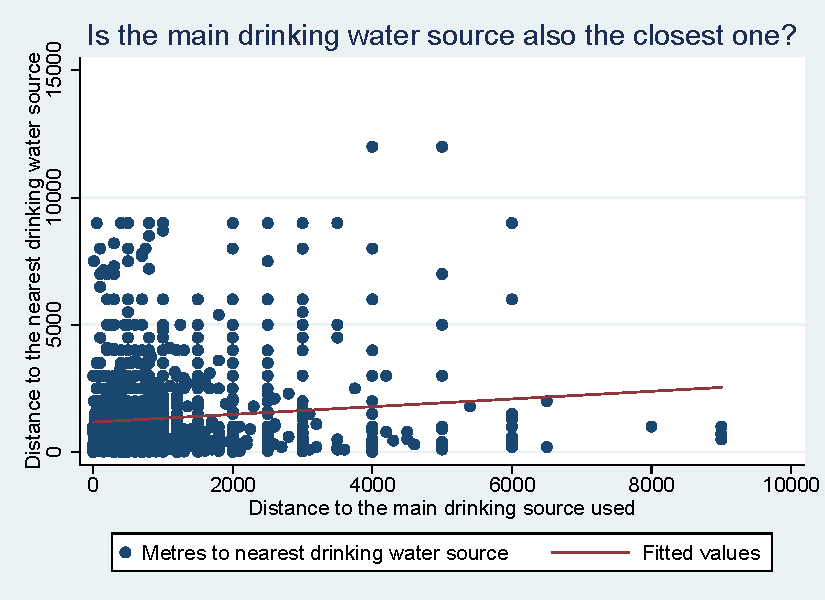
\includegraphics[width=0.8\textwidth]{scatter_1.pdf}
\end{center}
	\end{frame}
	
	\begin{frame}
	\frametitle{\textsc{Scatter plot}}	
		\onslide<1-> Let's make a scatter plot from your do file.
		\begin{enumerate}
			 \item Type \textbf{\textit{help scatter}} in the command window to find out what command to be used.
			 \onslide<2-> \item The command should look like the following. Run from the do file.
		
\begin{stlog}. quietly use "$data\\cs_s0_s5_household.dta", clear
>  
{\smallskip}
. quietly rename s5cq2 m_main_ws
{\smallskip}
. gen  km_main_ws = m_main_ws/1000
(1,098 missing values generated)
{\smallskip}
\end{stlog}
			\vspace{1mm}
			\onslide<3-> \item Notice the difference from earlier? No fitted line!
			\vspace{1mm}
		
\begin{center}
    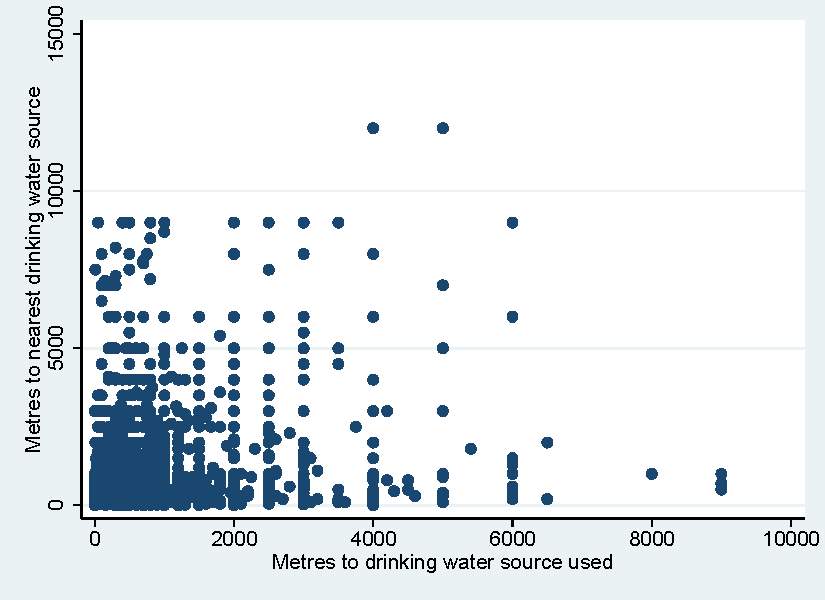
\includegraphics[width=0.5\textwidth]{scatter_2.pdf}
\end{center}
		\end{enumerate}
	\end{frame}
	
	\begin{frame}
	\frametitle{\textsc{Scatter plot}}	
		\onslide<1-> Let's add a fitted line. Type \textbf{\textit{help lfit}} to learn how to do this.
		\begin{enumerate}
			 \onslide<2-> \item You may notice that this is an entirely different command. 
								Stata can actually overlay multiple twoway graphs. 
								To do this, run the following command.
								Notice that \textbf{$\Vert$} is a way to overlay the graphs.
		
\begin{stlog}scatter m_used_ws m_drink_ws  || ///
lfit m_drink_ws m_used_ws
\end{stlog}
			\vspace{1mm}
			\onslide<3-> \item Notice the difference from earlier? No main title and y and y titles!
			\vspace{1mm}
		
\begin{center}
    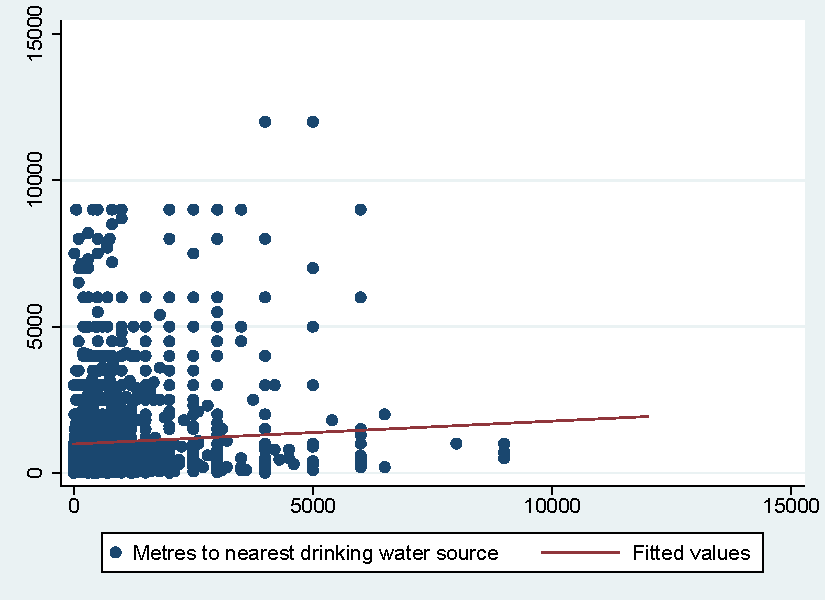
\includegraphics[width=0.5\textwidth]{scatter_3.pdf}
\end{center}
		\end{enumerate}
	\end{frame}

	\begin{frame}
	\frametitle{\textsc{Scatter plot}}	
		\onslide<1-> This is because the fitted line is a linear prediction and 
					 no longer represents the raw distance values. 
					 But we can simply add on titles that can be helpful for the graph's intended audience.
		\begin{enumerate}
			 \onslide<2-> \item Recall the \textbf{\textit{twoway\_options}}, and the \textbf{\textit{title()}} option.
								You can use the same option and very similar options called \textbf{\textit{xtitle()}} and
								\textbf{\textit{ytitle()}}.
		
\begin{stlog}export excel using "$data\\cs_s0_s5_household_modified.xls", /
> //
replace firstrow(variables)
\end{stlog}
		\end{enumerate}
	\end{frame}
	
	\begin{frame}
	\frametitle{\textsc{Stata graph exercise 3}}
		\begin{center}
		\Large \textbf{Saving and combining graphs}
		\end{center}
	\end{frame}	
	
	\begin{frame}
	\frametitle{\textsc{Saving a Stata graph}}
		Let's save all 3 graphs we made today.
		\begin{enumerate}
			\item To do so, add \textbf{\textit{graph save}} after each of your graphs like the following.
	
			\item Notice that you need to specify where you want save it,
				  and how you want to name it.
		\end{enumerate}
	\end{frame}
	
	\begin{frame}
	\frametitle{\textsc{Combining Stata graphs}}
		Let's combine all 3 graphs we made today.
		\begin{enumerate}
			\item To do so, add \textbf{\textit{graph combine}} after each of your graphs like the following.
	
			\item Notice that you need to specify where you want save it,
				  and how you want to name it.
		\end{enumerate}
	\end{frame}
	
	\begin{frame}
	\frametitle{\textsc{Combining Stata graphs}}
		\onslide<1-> Does yours look like this?
	
\begin{center}
    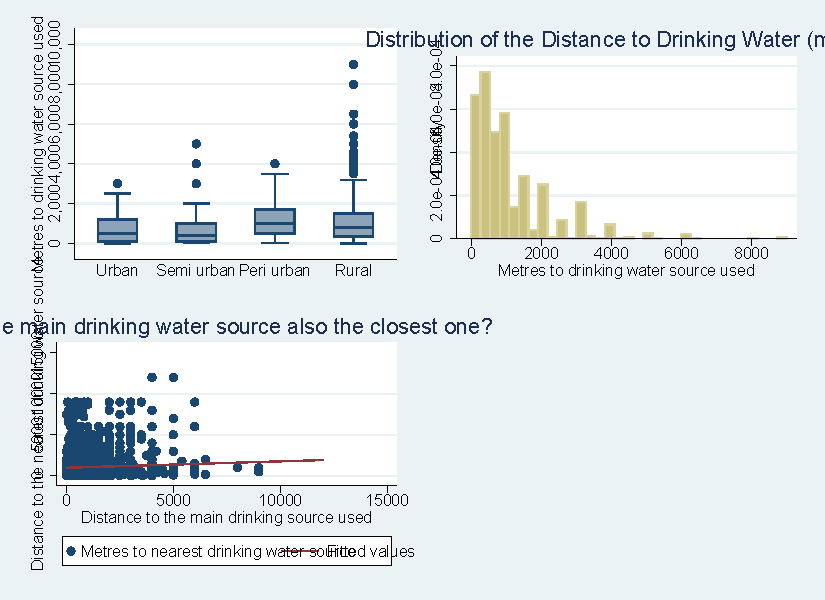
\includegraphics[width=0.5\textwidth]{combined.pdf}
\end{center}
		\begin{itemize}
			\onslide<2-> \item Why look so ugly?
			\onslide<3-> \item Luckily, there are ways to make this nice like this.			
		\end{itemize}
	\end{frame}
				
	\begin{frame}
	\frametitle{\textsc{Combining Stata graphs}}
		There are many ways to make it look better like the following. \\
		The solution do file will contain the commands to make the below graph. \\
		Change it around and have fun with it! \\
		Remember help files are your best friend.
	
\begin{center}
    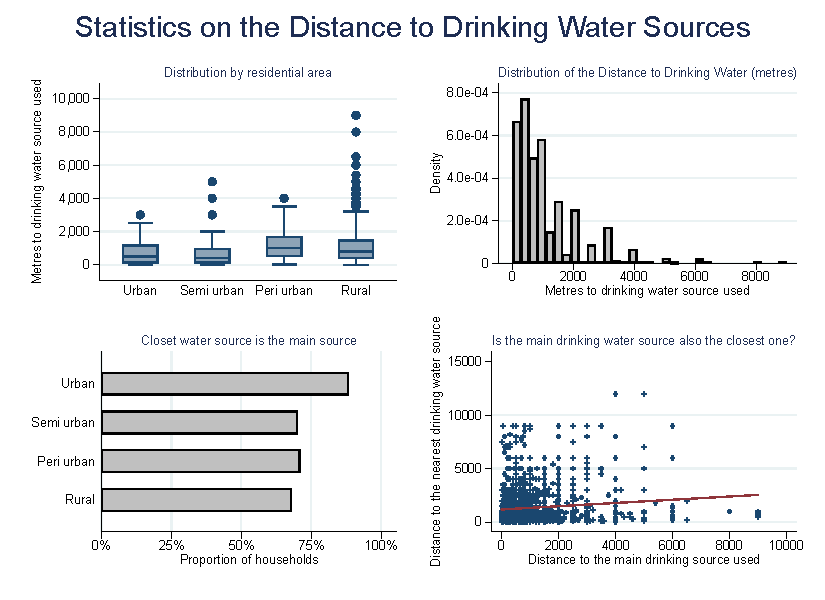
\includegraphics[width=0.5\textwidth]{combined_better.pdf}
\end{center}
	\end{frame}

				
	\section{Extra section: More about Stata}
	
	\begin{frame}
	\frametitle{\textsc{Other features of Stata}}
		\begin{center}
		\Large \textbf{Using macros \\ (globals, locals and scalars)}
		\end{center}
	\end{frame}

	\begin{frame}
	\frametitle{\textsc{Other features of Stata}}
		\begin{center}
			\LARGE \textbf{Macros}
		\end{center}
		\begin{itemize}
			\item You need to be at least familiar with this topic for 
				  the resources you will be introduced to this week
			\item This technique is critical as projects grow in size. 
				  But even the smallest DIME project absolutely needs this.
			\item Macros (globals, locals, scalar) save some information 
				 (text or number) that you can reference later.
				\begin{itemize}
					\item Example: we want to access files in the folder 
								   multiple times. We can store the folder 
								   location in a global and use it multiple times
				\end{itemize}
		\end{itemize}
	\end{frame}

	\begin{frame}
	\frametitle{\textsc{Other features of Stata}}
		\begin{center}
			\onslide<1-> \LARGE \textbf{Defining macros - local}
		\end{center}
		Type in your dofile the following and \textit{run all the lines at once}.
		\begin{itemize}
			\item Note that \textbf{`} is not the same as \textbf{'}.
\begin{stlog}graph box m_drink_ws, over(urban_2012)
\end{stlog}
		\vspace{2mm}
		\onslide<2-> \item What did the result say?
		\onslide<3-> 
\begin{stlog}The result is 12.
{\smallskip}
\end{stlog}
			\onslide<4-> \item Try running them one by one, and see what happens?
				\begin{itemize}
					\onslide<5-> \item It probably didn't run. 
									   This is one of the major differences between global and local.
									   Local is really local and only last within a single run.
									   For more please refer to the help file on \textit{macro}.
				\end{itemize}
		\end{itemize}
	\end{frame} 
	
	\begin{frame}
	\frametitle{\textsc{Other features of Stata}}
		\begin{center}
		\Large \textbf{Missing values}
		\end{center}
	\end{frame}
		
	
	\begin{frame}
	\frametitle{\textsc{Other features of Stata}}
		\begin{center}
			\LARGE 	\textbf{Missing values}
		\end{center}
		\begin{itemize}
			\item String variables can be empty, but numeric variables can’t be empty. 
				  Instead numeric variables have something called “missing values”.
				\begin{itemize}
					\item Missing values are represented in Stata with a period as in " \textbf{.} ". 
					\item You can also use .a or .b etc. to .z for missing values 
						  and you will learn later how these can be used
				\end{itemize}
			\item Stata can’t use missing values in computations (averages, regressions etc.) 
				  so it skips observations with missing values . 
			\item Missing values changes the analysis as observations with 
				  missing values are excluded from commands like summarize and regress.
			\item Good practice to always check for missing values when tabulating variables.			
		\end{itemize}
	\end{frame}
	
	\begin{frame}
	\frametitle{\textsc{One more useful command}}
		\begin{center}
		\Large \textbf{tabstat: \\ another command of summary statistics}
		\end{center}
	\end{frame}
		
	\begin{frame}
	\frametitle{\textsc{One more useful command}}
		\begin{center}
			\LARGE \textbf{tabstat}
		\end{center}
		\begin{itemize}
			\item While \textbf{\textit{summarize}} and \textbf{\textit{tabulate}} 
				  provide useful fixed format output, 
				  \textbf{\textit{tabstat}} gives you the ability specify 
				  exactly what statistics you want in your input.
			\item By default, \textbf{\textit{tabstat}} only disply the mean.
			\item We can add a whole range of statistics using the option 
				  \textbf{\textit{statistics()}}. 
				  See \textbf{\textit{help tabstat}}, for a list of the statistics you can add.
		\end{itemize}
	\end{frame}
	
	\begin{frame}
	\frametitle{\textsc{One more useful command}}
		Here are some examples.
		\begin{itemize}
			\item This is the very basic command.
\begin{stlog}. tabstat m_main_ws m_used_ws
{\smallskip}
   stats {\VBAR}  m_main{\tytilde}s  m_used{\tytilde}s
\HLI{9}{\PLUS}\HLI{20}
    mean {\VBAR}  791.2462   863.863
\HLI{9}{\BOTT}\HLI{20}
{\smallskip}
\end{stlog}
			\vspace{2mm}
			\item You can add multiple variable at a time.
\begin{stlog}histogram m_drink_ws, ///
title("Distribution of the Distance to Drinking Water (metres)")
\end{stlog}
		\end{itemize}
	\end{frame}
		
	\begin{frame}
	\frametitle{\textsc{One more useful command}}
	Lastly...
		\begin{itemize}
			\vspace{2mm}
			\item You choose what types of statistics you want it to display.
\begin{stlog}histogram m_drink_ws, ///
title("Distribution of the Distance to Drinking Wat
> er (metres)")
\end{stlog}
		\end{itemize}
	\end{frame}
	
	\end{document}
